%-----------------------------------------------------------------------------------------------
\documentclass[addpoints, 11pt]{exam}
\usepackage[margin=.75in]{geometry}
\usepackage{etex}
\usepackage{graphicx}
\usepackage{amssymb}
\usepackage[fleqn]{amsmath}
\usepackage{nccmath}
\usepackage{cases}
\usepackage{hyperref}
\usepackage{multicol}
\usepackage{enumerate}
\usepackage{tikz}
\usepackage{pgfplots}
\usetikzlibrary{patterns}
\usepackage{pstricks-add}
%\usepackage{pst-func}
%\usepackage{pst-plot}
%\usepackage{pst-spectra}
\usepackage{multido}
\usepackage{lastpage}
\usepackage{ulem}
\usepackage[outside]{coordsys}
\usepackage{float}
\usetikzlibrary{pgfplots.statistics}
\usetikzlibrary{positioning, shapes.geometric}
%-------------------------------------------------------------------------------------------------
\setlength{\columnsep}{.5cm}
\setlength{\columnseprule}{1pt}
\newcommand{\ds}{\displaystyle}
\newcommand{\work}{{\bf{No Work $\Leftrightarrow$ No Points }}}
\newcommand{\neat}{{\bf{Use Pencil Only $\Leftrightarrow$ Be Neat \& Organized }}}
\newcommand{\answer}{\large\bf Ans: \underline{\hspace{1.5in}}}
\newcommand{\la}{\lambda}
\newcommand{\zz}{\mathbb{Z}}
\newcommand{\rr}{\mathbb{R}}
\newcommand{\nn}{\mathbb{N}}
\newcommand{\qq}{\mathbb{Q}}
\newcommand{\cc}{\mathbb{C}}
\newcommand{\cyclic}[1]{\langle #1 \rangle}
\newcommand{\lcm}{{\rm{lcm}}}
\renewcommand{\solutiontitle}{\noindent\textbf{Answer:}\par\noindent}
%------------------------------------------------------------------------------------------------
\begin{document}
%------------------------------------------------------------------------------------------------
\cfoot{UCLA: C. Johnson}
%	\rfoot{Total Points: \numpoints}
\rfoot{Page \thepage\ of \pageref{LastPage}}
%------------------------------------------------------------------------------------------------
\begin{center}
\fbox{%
	\parbox{1\linewidth}{%
		\noindent \Large\bfseries \\[.05in] Math 142: Modeling{\hspace{1.2in}{\Large\bfseries Name:{\hrulefill}}\\[.2cm]
			\noindent \Large\bfseries Homework \# 2 \hspace{2.8in}{Due:} Friday Oct 13
		}\\[.025in]
	}%
}
\end{center}
\addpoints


\vspace{.25cm}


%------------------------------------------------------------------------------------------------
\noindent  {\bf Directions} Complete the exercises. Your solutions to the exercises should be submitted to Gradescope before the indicated due date above. Please follow rules regarding Gradescope submission as described in the syllabus. \\


\noindent{\bf References} Except for the help of the instructor or TAs and the class textbooks and notes, if you use any resources, for example, a book, a website, or you discussed with your friends, please acknowledge them in this References section. 
\begin{itemize}
\item I discussed Problem ?? with STUDENT A, STUDENT B, $\ldots$
\item I used BOOK/WEBSITE to help me do Problem ??.
\end{itemize}
\vspace{.05cm}
%\hrule
%----------------------------------------------------------------------------------------------  
\noindent {\bf Exercises}
%\begin{multicols*}{2}
\begin{questions}
%----------------------------------------------------------------------------------------------  
\question  Look at the mathematical model for the growth of the red wolf population, when wild born and introduced wolves were considered in the last homework. 
\begin{parts}
	\part In addition to the wild red wolf population there is a captive breading population. One strategy is to introduce captive bred wolves into the wild. Suppose that 10 captive bread wolves are added to the wild population each year. Unfortunately, captive bred wolves do not readily integrate into existing packs, and are less effective hunters than wild-born wolves. As a result $43 \%$ of introduced wolves die each year. To model the effect of introducing wolves, we must keep track of both the number of wild-born wolves, $N_t$ and the number of wolves that are introduced $I_t$.
	\begin{enumerate}[(i)]
		\item Explain why:
		$$
		\begin{aligned}
			N_{t+1} &=1.06 N_t+0.28 I_t \\
			I_{t+1} &=10+0.57 I_t
		\end{aligned}
		$$
		(explain what each term in the equations represents). Also explain why the total number of wild red wolves is given by $N_t+I_t$\\

		Given the number of wild wolves at time $t$ is $N_t$ and the number of captive bred wolves at time $t$ is $I_t$, the total number of wolves would be the sum of the two populations i.e $N_t+I_t$.
		Let $b_c=0.28$ be the birth rate of the captive bred wolf population. Since the $0.28I_t$ wolves born at time $t$ are born in the wild, they will be a part of the wild wolf population at time $t+1$.
		Let $R_0=b_w-m_w=0.06$ be the net reproduction rate of the wild wolf population. 
		Thus, the number of wild wolves at time $t+1$ $(N_{t+1})$ is the sum of the number of wolves at time $t$ $(N_t)$, the number of wild wolves born from wild parents minus the number of wild wolves that died at time $t$ $(R_0N_t=(b_w-m_w)N_t)$, and the number of wild wolves born from captive bred parents $(b_cN_t)$.
		Let $m_c=0.43$ be the mortality rate for captive bred wolves. Let $r=10$ be the number of captive bred wolves introduced each year. 
		Thus, the number of captive bred wolves at time $t+1$ $(I_{t+1})$ is the sum of the number of captive bred wolves at time $t$ minus the number of captive bred wolves that died at time $t$ $((1-m_c)I_t)$ and the number of captive bred wolves introduced at time $t$ $(r)$.
		\item Calculate $N_t$ and $I_t$ for $t=0,1,2,3,4,5$, assuming that $N_0=130$ and $I_0=0$. Then, using Matlab, or by some other means, calculate when the total number of wild red wolves will reach the target population size of 220.\\
		
		The population will first the $220$ wild wolf threshold at $t=7$.\\
		\begin{figure}[h]
			\centering
			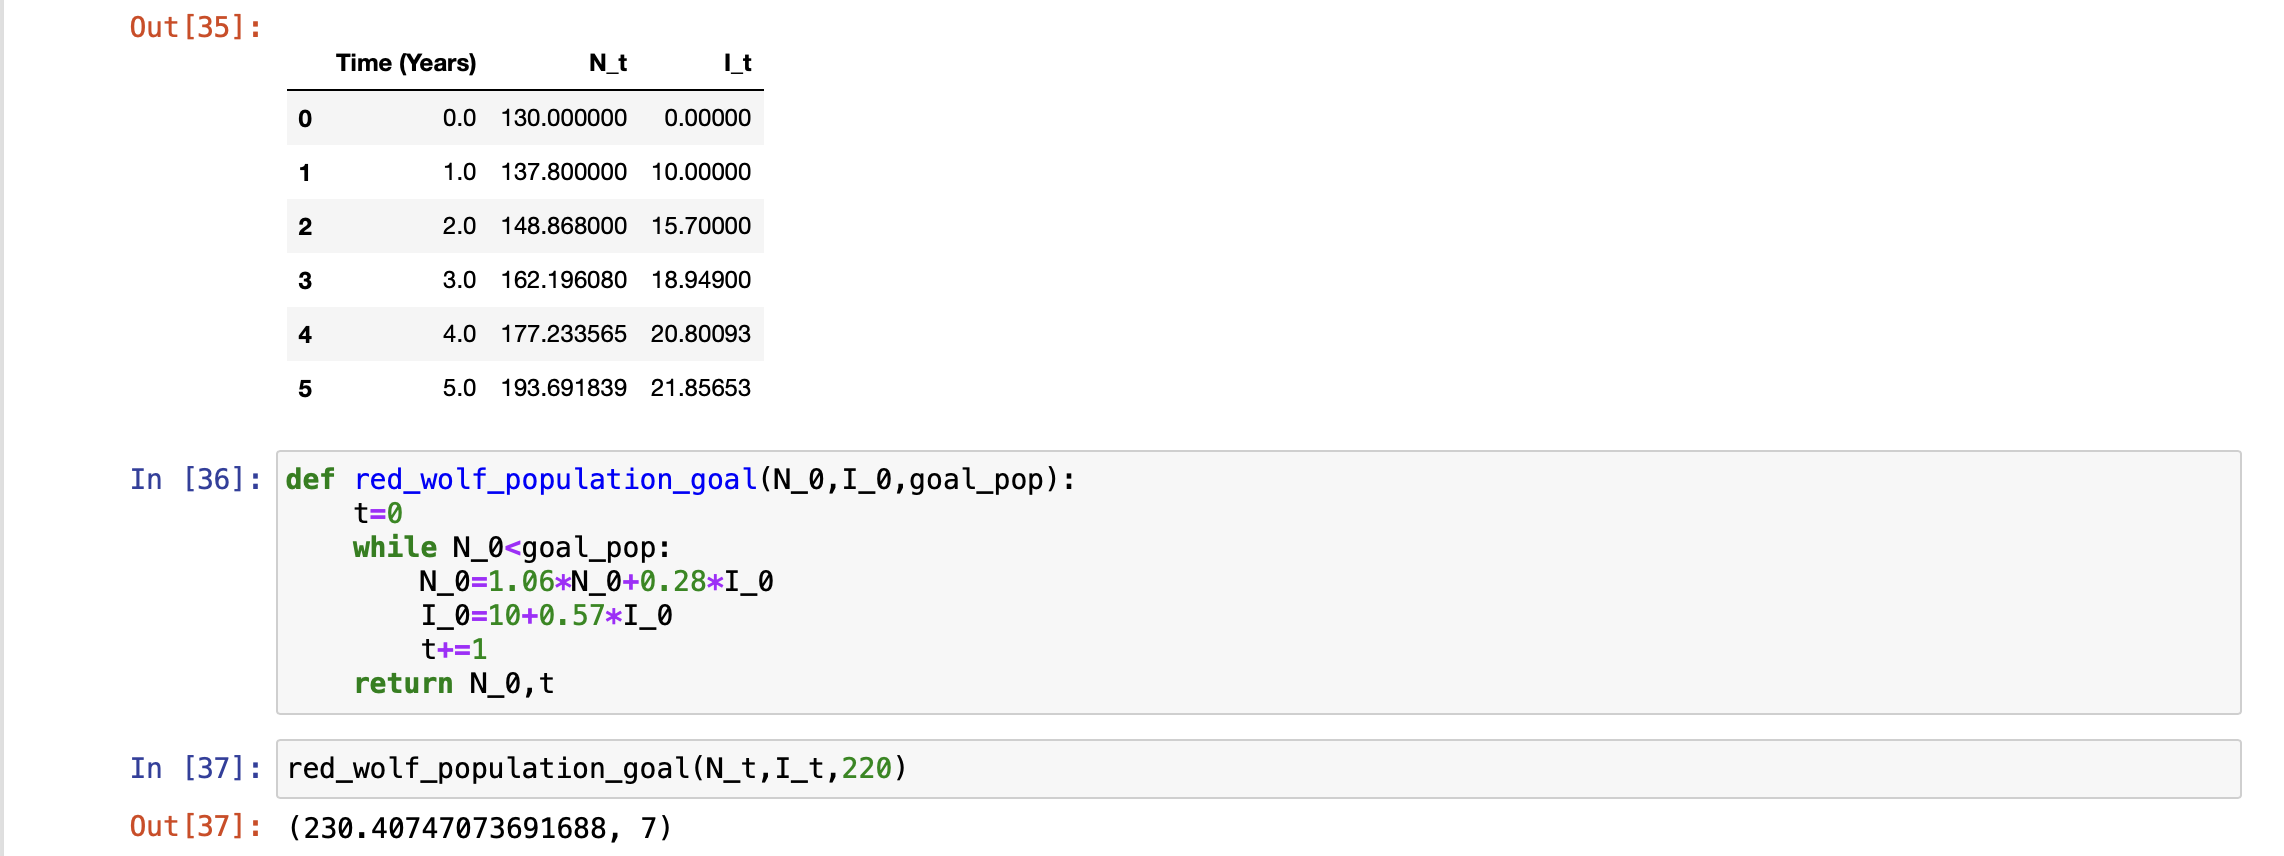
\includegraphics[scale=0.4]{Screenshot 2023-10-11 at 3.13.06 PM.png}
		\end{figure}
		\item Make a plot of how the population size grows as a function of $t$. Show that the growth is eventually exponential.\\
		\begin{figure}[h]
			\centering
			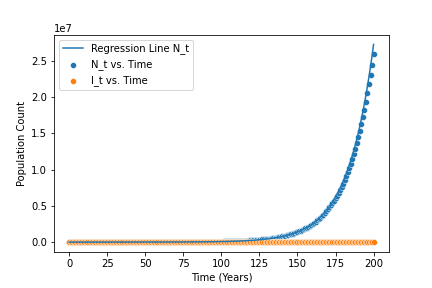
\includegraphics[scale=0.4]{Math_142_Homework_2_Q_1_a.png}
		\end{figure}
		As $t$ grows large, the plot of $N_t$ vs. time appears to closely follow the exponential regression graph.\\
	\end{enumerate}
	\part Explain why the recurrence equations that you derived for $I_t$ and $N_t$ can not be written as an iterated linear map (i.e. using a Leslie matrix) - identify the specific term(s) that can not be represented using the Leslie matrix.\\
	
	Every generation, $I_{t+1}$ depends a constant number of captive bred wolves added to the population. This constant quantity is independent of $I_t$ and $N_t$ and therefore can't be expressed in Leslie matrix from.
	\part For the Leslie matrix:
	$$
	L=\left(\begin{array}{cc}
		1 & 3 / 2 \\
		2 & 1 / 2
	\end{array}\right)
	$$
	\begin{enumerate}[(i)]
		\item Assume that you have initial data: $\mathbf{N}^{(0)}=\left(\begin{array}{l}100 \\ 200\end{array}\right)$. Calculate by hand, or using a computer, $\mathbf{N}^{(k)}$ for $k=1,2,3$.\\
		\begin{figure}[h!]
			\centering
			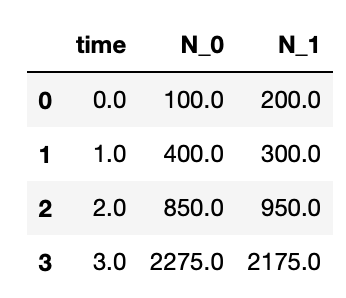
\includegraphics[scale=0.6]{Screenshot 2023-10-12 at 4.48.24 PM.png}
		\end{figure}

		\item Verify that $\left(\begin{array}{l}1 \\ 1\end{array}\right)$ is an eigenvector of the Leslie matrix, and find the corresponding eigenvalue. Then derive a formula for the subpopulation sizes at arbitrary $k$ if $\mathbf{N}^{(0)}=\left(\begin{array}{l}100 \\ 100\end{array}\right)$.\\
		$\left(\begin{array}{cc}
			1 & 3 / 2 \\
			2 & 1 / 2
		\end{array}\right)
		$
		$\left(\begin{array}{l}1 \\ 1\end{array}\right)=\left(\begin{array}{l}2.5 \\ 2.5\end{array}\right)$
		Thus, $2.5$ is an eigenvalue, and $\mathbf{N}^{(k)}=(2.5)^k\mathbf{N}^{(0)}$
	\end{enumerate}
	\part For the Leslie matrix:
	$$
	L=\left(\begin{array}{cc}
		11 / 2 & 3 / 2 \\
		3 / 2 & 3 / 2
	\end{array}\right)
	$$
	find both of the eigenvalues and the corresponding eigenvectors. Explain why there is at least one initial condition for which a model using this matrix would predict unbounded exponential growth.\\
	$\det(L-x\cdot I)=(6-x)(1-x)=0$ for $x=6,1$\\
	$L\left(\begin{array}{l}3 \\ 1\end{array}\right)=\left(\begin{array}{l}18 \\ 6\end{array}\right)$\\
	$L\left(\begin{array}{l}-1 \\ 3\end{array}\right)=\left(\begin{array}{l}-1 \\ 3\end{array}\right)$\\
	There exists a dominant eigenvalue $\lambda=6$, so the sub-populations will grow exponentially as $t$ becomes large by a factor of $6$ assymptotically approaching the line in the direction of the $\left(\begin{array}{l}3 \\ 1\end{array}\right)$ vector.
	\part For the Leslie matrix:
	$$
	L=\left(\begin{array}{cccc}
		5 & 1 & 1 & 0 \\
		3 / 2 & 1 / 2 & 0 & 1 \\
		0 & 1 / 2 & 0 & 0 \\
		0 & 0 & 1 / 4 & 0
	\end{array}\right)
	$$
	show, without directly computing the eigenvalues of $L$, that there is an eigenvalue larger than 1 , so the population will grow exponentially.\\
$\det(L-1\cdot I)=\frac{-15}{4}<0$\\
Because L's characteristic polynomial is $4th$ degree with a leading coefficient of $1$. $(5-x)(1-x)(-x)(-x)=x^4+\ldots$ is the only diagonal contributing to the fourth degree term. Since $\det(L-1\cdot I)<0$ and $\det(L-xI)$ is increasong for all $x>1$, $\det(L-xI)$ must have a root for some $x>1$ by the IVT.
\begin{figure}[H]
	\centering
	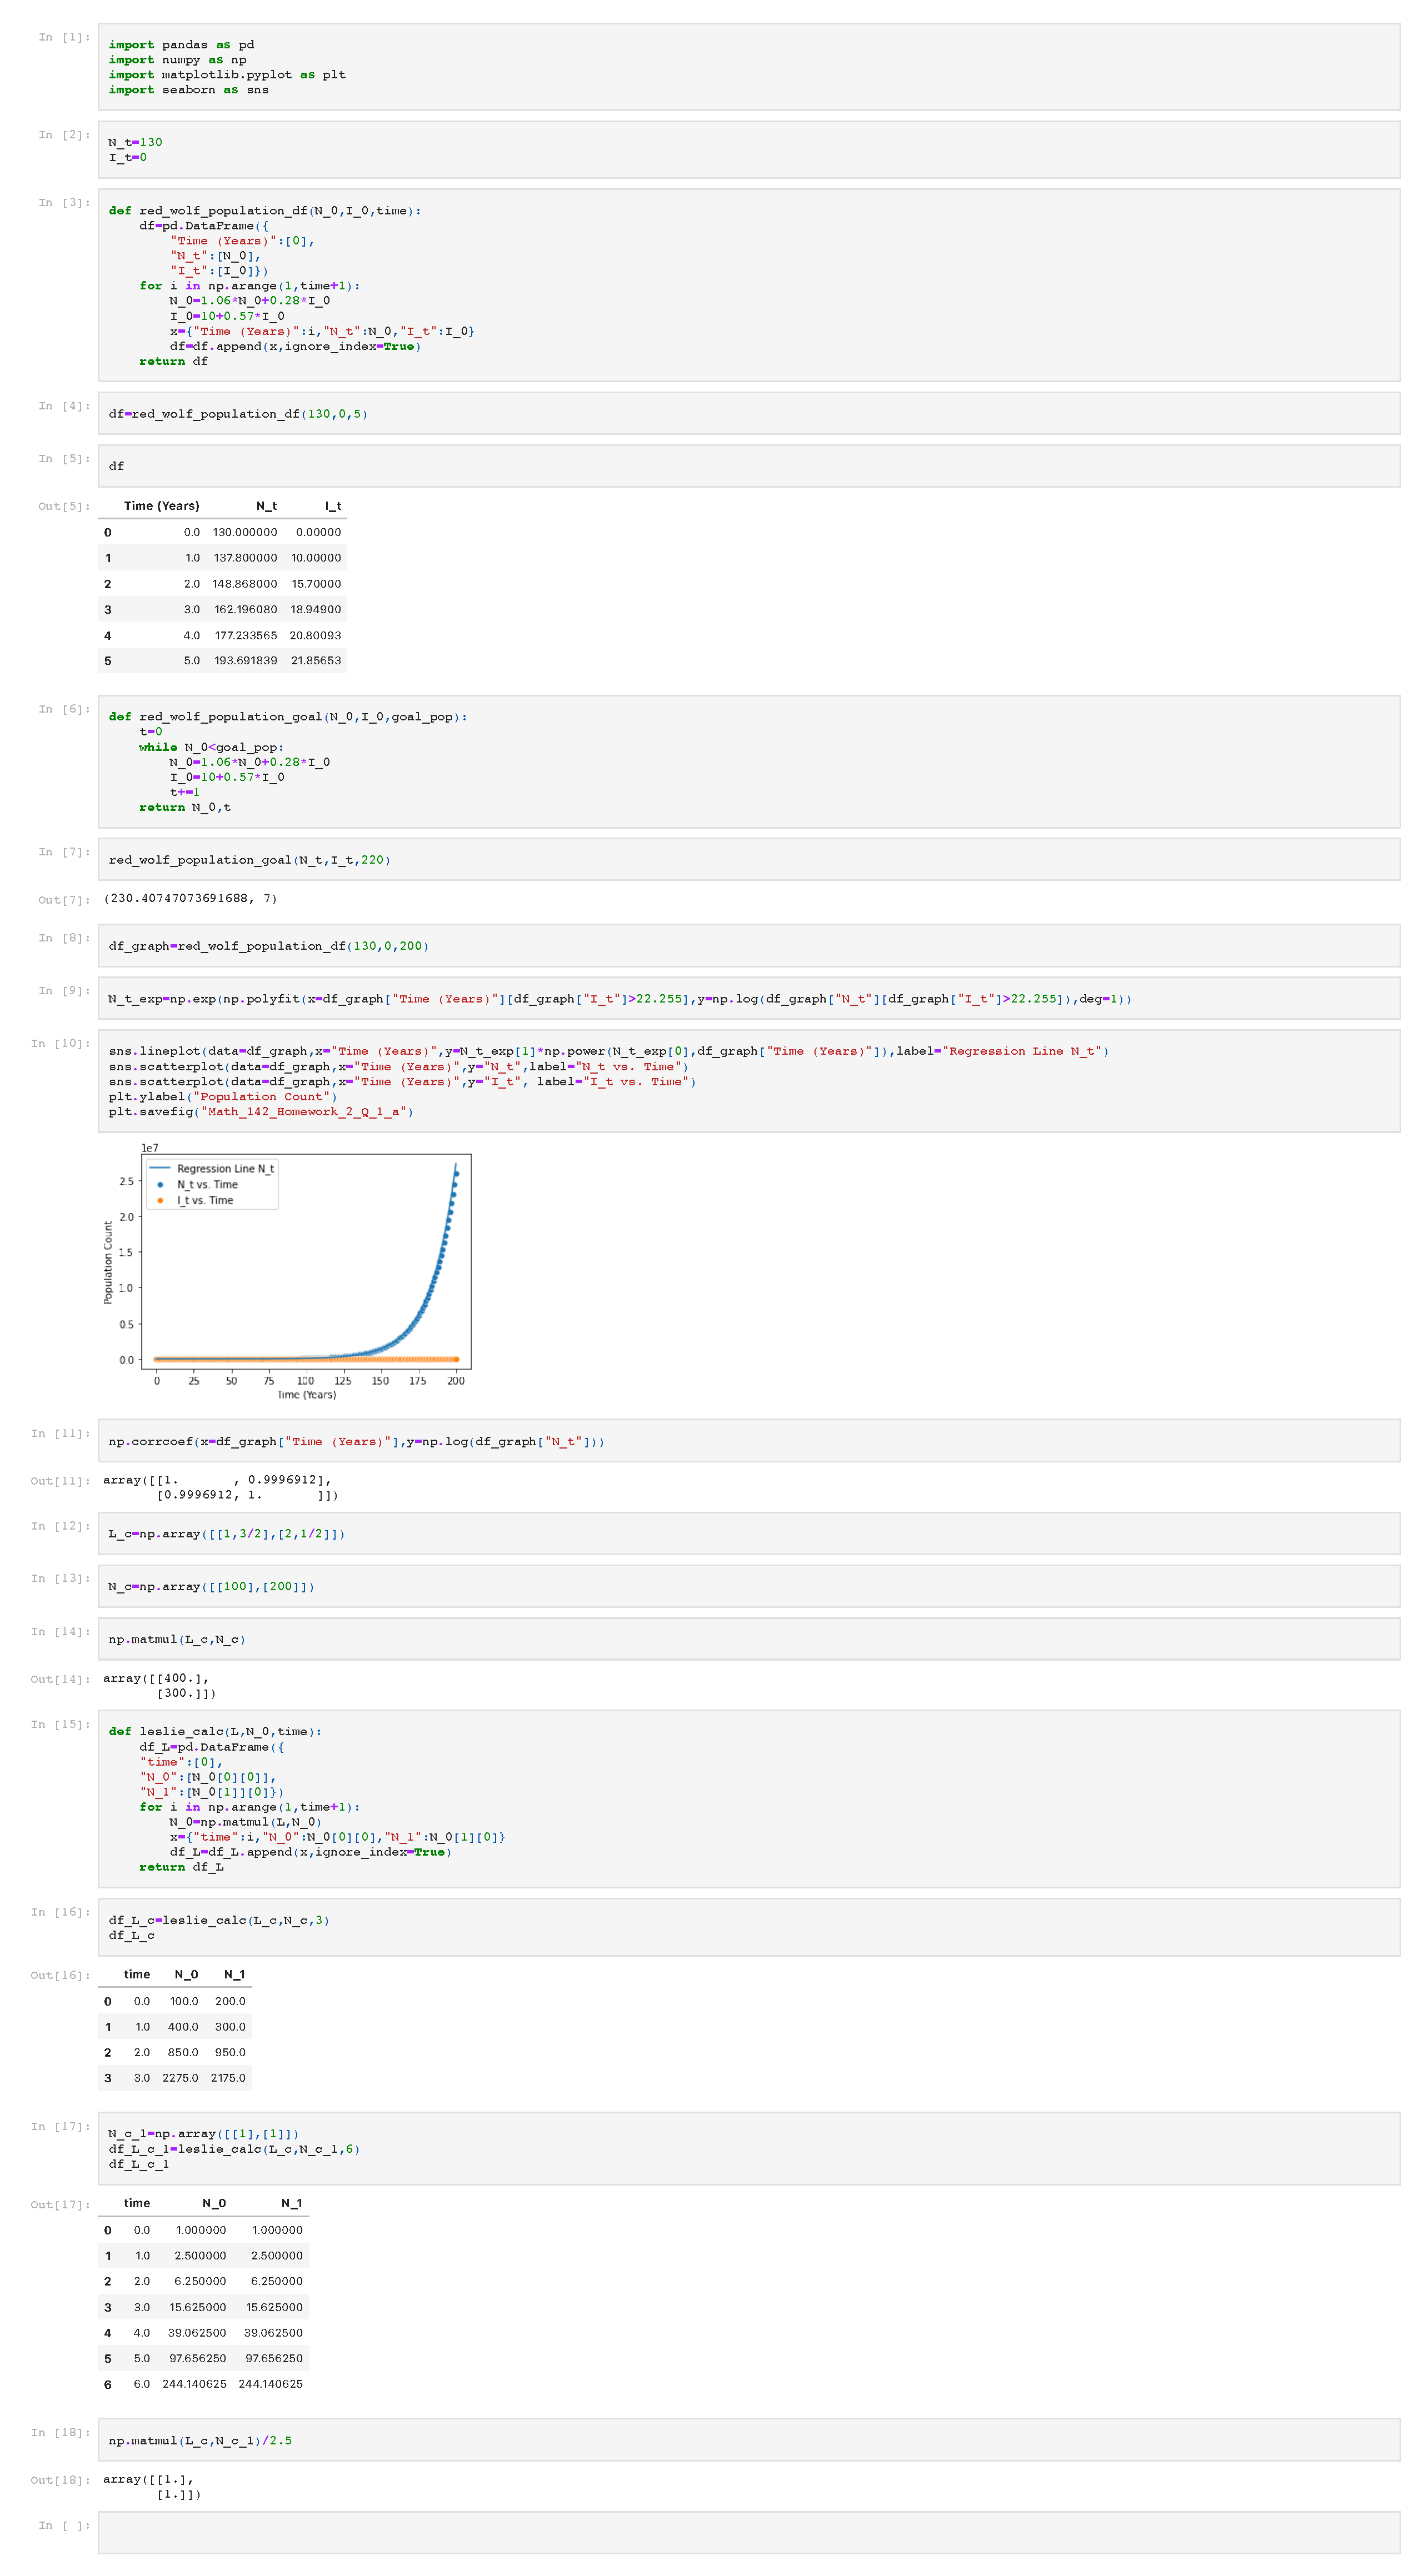
\includegraphics[scale=0.3]{Math_142_Homework_2_Q_1.pdf}
\end{figure}
\end{parts}
%----------------------------------------------------------------------------------------------   
\question A drug in which the amount of drug is eliminated is constant. At time $t=0$ an amount $a_0=20$mg is present in the blood. One hour later, at $t=1$, an amount $a_1=14$mg is present.
\begin{parts}
	\part Assuming that no drug is added to the blood between $t=0$ and $t=1$, calculate the amount of drug that is removed from the blood each hour.\\

	$a_0-a_1=20-14=6$ $6$mg are removed each interval.
	\part Write a recursion relation for the amount of drug $a_t$ that is present at time $t$. Assume no extra drug is added to the blood.\\

	$a_{t+1}=\max(0,a_t-6)$
	\part Find an explicit formula for $a_t$ as a function of $t$.\\
	
	$a_t=\max(a_0-6t,0)=\max(20-6t,0)$
	\part When does the amount of drug present in the blood first drop to 0?\\

	$2-6\cdot3=2,20-6\cdot4=-4$, so drug first reaches $0$ when $t=4$.
\end{parts}
%----------------------------------------------------------------------------------------------
\question We want to model painkillers that are absorbed into the blood from a slow release pill. Our mathematical model for the amount, $a_t$, of the drug in the blood $t$ hours after the pill is taken must include the amount absorbed from the pill each hour. Assume that the amount absorbed from the pill between time $t$ and the time $t+1$ is $\ds10\cdot(0.4)^t$.
\begin{parts}
	\part The amount of drug is eliminated depends on the amount in the system. $10\%$ of the drug is eliminated from the blood each hour. Write down the recursion relation for $a_{t+1}$ in terms of $a_t$.\\

	$a_{t+1}=10\cdot{(0.4)}^t+0.90\cdot a_t$
	\part Assuming that $a_0=0$, meaning that no drug is present in the blood initially, calculate the amount of drug present at times $t=1,2,\ldots,6$.\\
	\begin{figure}[H]
		\centering
		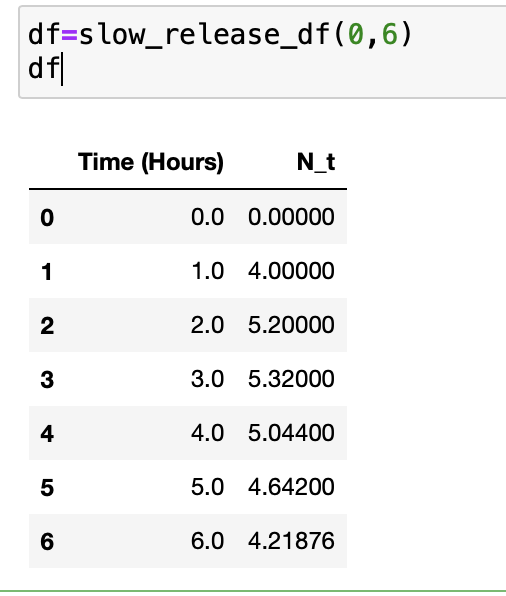
\includegraphics[scale=0.3]{Screenshot 2023-10-12 at 12.50.53 PM.png}
	\end{figure}
	\part What is the maximum amount of drug present at any time in this interval? At what time is this maximum amount reached?\\
	$N_3=5.32$ at $t=3$
	\part Use a computer to calculate the amount of drug present in hourly intervals from $t=0$ up to $t=24$.\\
	\begin{figure}[H]
		\centering
		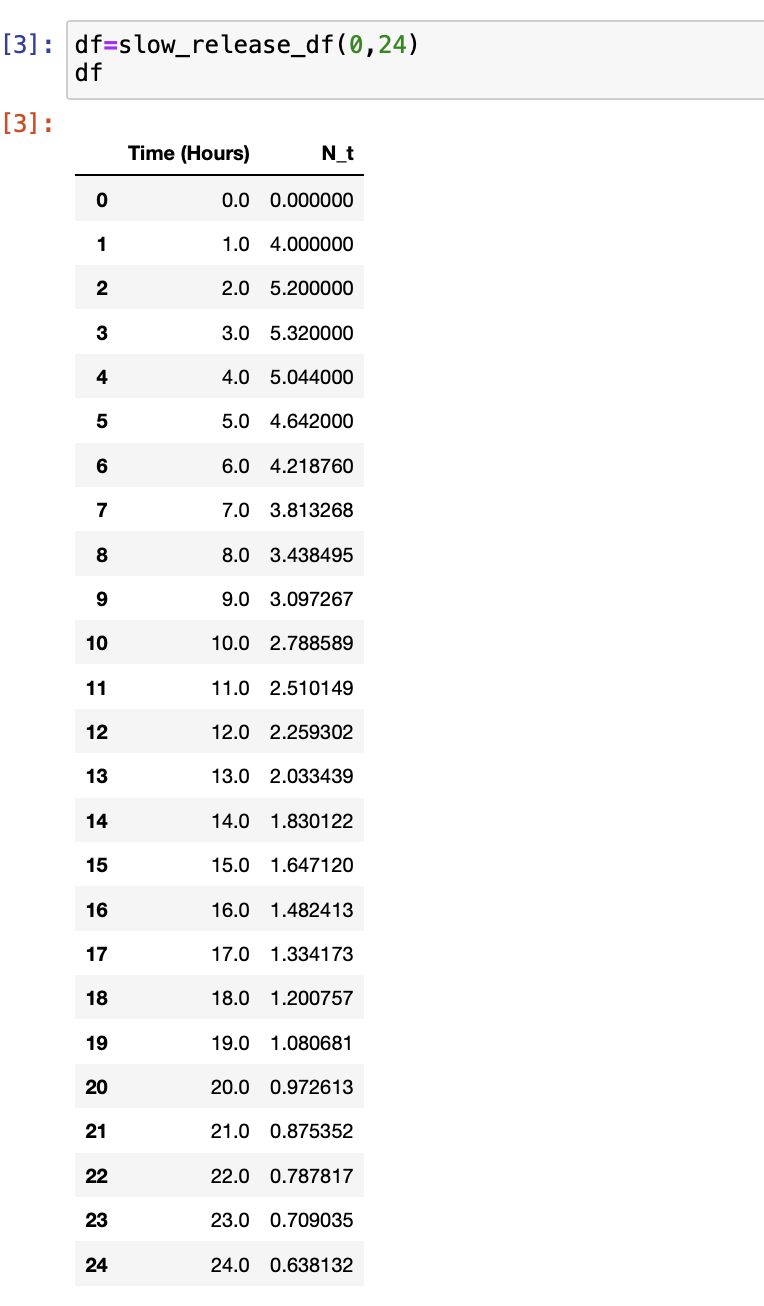
\includegraphics[scale=0.3]{Screenshot 2023-10-12 at 8.09.19 PM.png}
	\end{figure}
	\item Show that when $t$ is large, the amount of drug present in the blood decreases approximately exponentially with $t$.\\
	\begin{figure}[H]
		\centering
		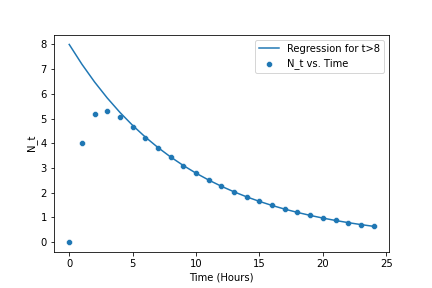
\includegraphics[scale=0.5]{Math_142_HW_2_Q_3a.png}
	\end{figure}
	\begin{figure}[H]
		\centering
		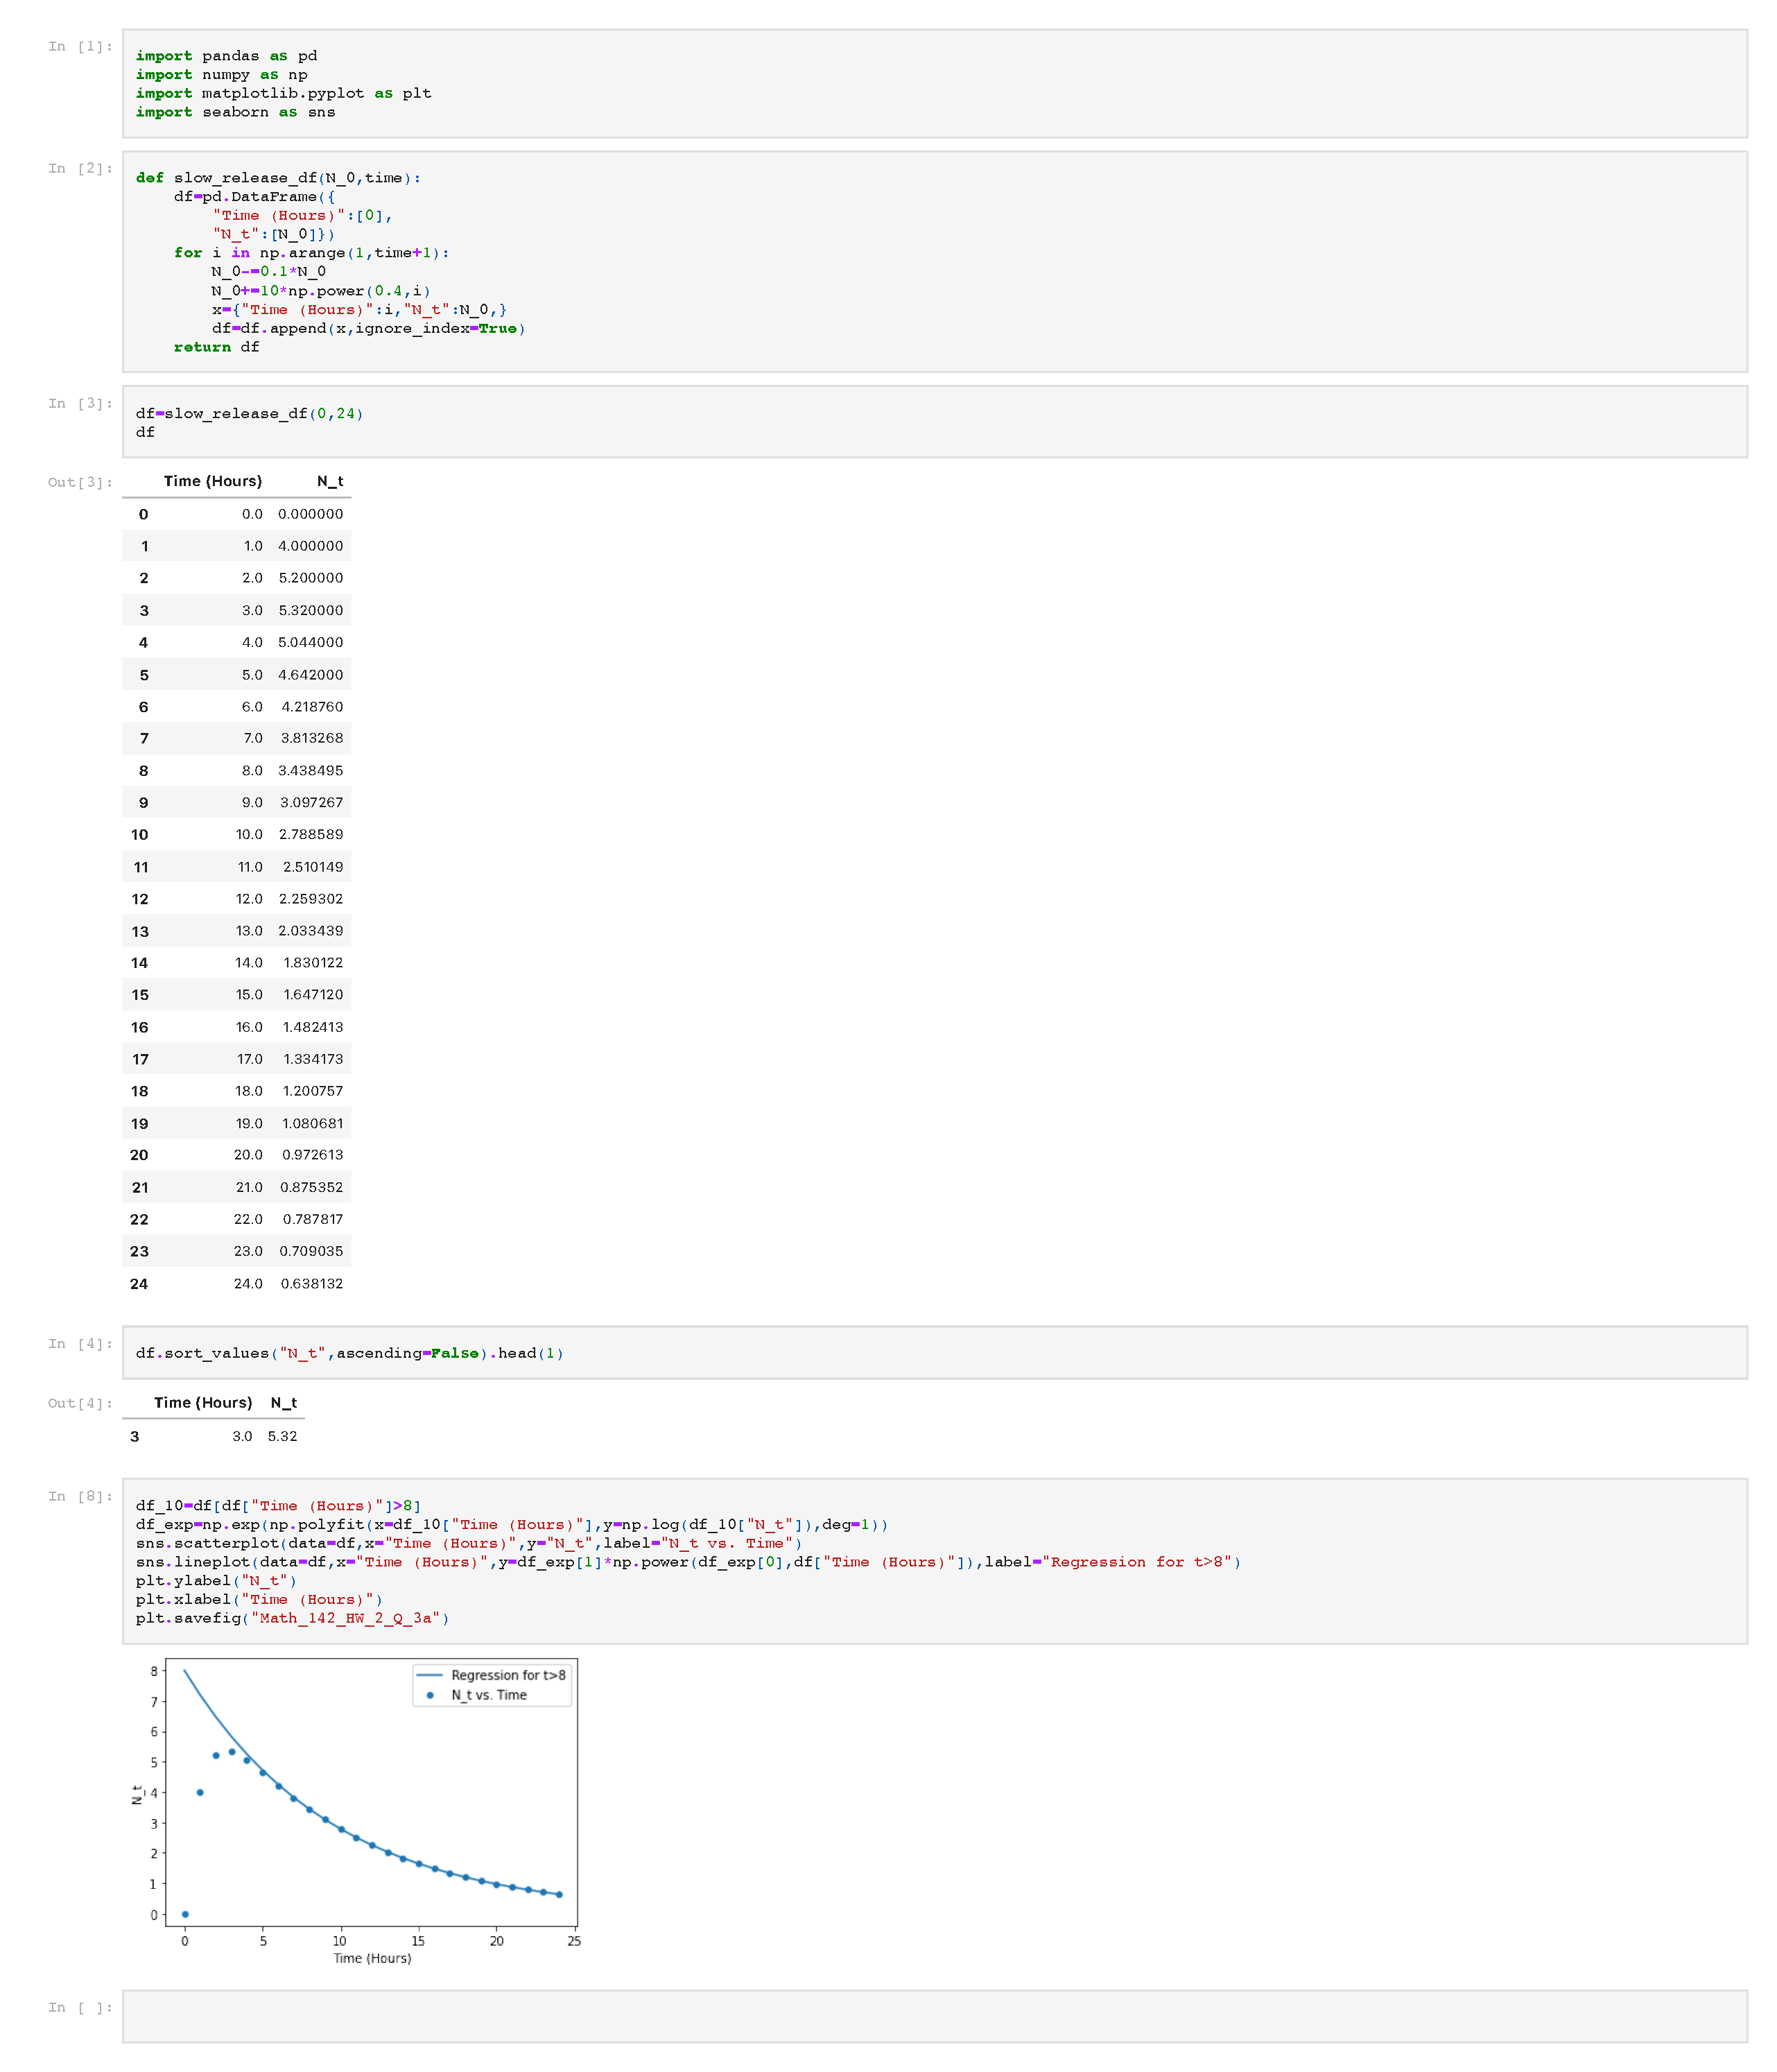
\includegraphics[scale=0.3]{Math_142_Homework_2_Q_3.pdf}
	\end{figure}
\end{parts}
%----------------------------------------------------------------------------------------------
%\question In this question we are going to create a Leslie matrix model for the US population. We will have to collect data of birth and death rates from the National Center for Health Statistics.\\
%
%\indent You can download the most recent (2017) data on mortality rates from:
%\url{ https://ftp.cdc.gov/pub/Health_Statistics/NCHS/Publications/NVSR/68_07/}\\
%
%\indent The different tables break the data down by race and by sex-at-birth. Table01 aggregates the data over the entire population. This is the table that we will use. The probability of dying data are all in column B.\\
%
%\indent For birth rates we will use the data from 2017 published in Table 2 (Page 13) of the report:
%
%\url{https://www.cdc.gov/nchs/data/nvsr/nvsr68/nvsr68_13-508.pdf}
%
%\indent One wrinkle - birth rates are reported for women, but our population model includes all individuals (including non-women). Assume that a fraction $0.508$ of individuals are women (also based on CDC data). So multiply birth rates by $0.508$ to account for the fact that we must find the fraction of individuals in the age group who are women, and then find the fraction of births.\\
%
%\indent Your first goal is to assemble a Leslie matrix using all of these data. For the birth rate data, which is aggregated over 5 years - e.g. 20-24 it is acceptable to assume that all ages in the group have the same birth rate - i.e. use the same birth rate for 20, 21, 22, 23 and 24 year olds. There is no need to write out or print the matrix - just use it to answer the questions.
%\begin{parts}
%	\part Why might it be inaccurate to assume that the same fraction of individuals in each age group are women? In other words why might different age groups have different fractions of women?
%	\part Use Matlab to calculate the largest eigenvalue of your matrix. Is it larger than 1, meaning that the population will increase over time?
%	\part Find for yourself the most recent data on the distribution of ages of individuals in the US (cite the website or source that you used). Using your Leslie matrix model, predict how the populations will grow or decay over the next 100 years. Demonstrate your answer by making the following plots:
%	\begin{enumerate}[(i)]
%		\item The total population over time.
%		\item The number of people over the age of 65 as a fraction of the total population size.
%		\item The number of college age (i.e. 18-25) people as a function of the total population size.
%	\end{enumerate}
%	\part What important effect did we miss when trying to predict demographic change in the US?
%\end{parts}
%----------------------------------------------------------------------------------------------   
\question  This question is about developing a model for the life-cycle of a type of nanoflagellates, a type of swimming cell that lives in water. The nanoflagellate cells go through three different life history stages. All cells start as swimming larvae (we call this the juvenile phase). They swim around looking for a surface (e.g. a plant) to settle on. When they settle they become tethered. Tethered cells feed for a while, and then when they have exhausted the food nearby they break their tethers, and start to swim around in search of another place to settle (we call these cells freely swimming). Only tethered cells are capable of reproducing. At all stages the organism can also die, in which case it won't transition to another stage. You are modeling for how the three populations vary with time: at the $k$ th census there are $N_F^{(k)}$ freely swimming cells, $N_J^{(k)}$ juvenile cells and $N_T^{(k)}$ tethered cells. Measurements are taken daily. Our model needs to incorporate the following information:
\begin{itemize}
	\item In each day, a fraction $m$ of cells in all of the stages die.
	\item Of the freely swimming cells that do not die, a fraction $t$ will become tethered.
	\item Of the tethered cells that do not die, a fraction $u$ will become untethered (i.e. enter the freely swimming phase).
	\item Of the tethered cells that do not die, a fraction $b$ will divide in two, producing a larval cell as a daughter.
	\item Of the juvenile cells that do not die, a fraction $c$ will become tethered.
\end{itemize}
\begin{parts}
	\part Show that the changes in this population from one census to another can be modeled by the following Leslie matrix:
	$$
	\left(\begin{array}{c}
		N_F^{(k+1)} \\
		N_J^{(k+1)} \\
		N_T^{(k+1)}
	\end{array}\right)=\left(\begin{array}{ccc}
		(1-m)(1-t) & 0 & (1-m)u \\
		0 & (1-m)(1-c) & (1-m)b \\
		(1-m)t & (1-m) c & (1-m)(1-u)
	\end{array}\right)\left(\begin{array}{c}
		N_F^{(k)} \\
		N_J^{(k)} \\
		N_T^{(k)}
	\end{array}\right)
	$$
	where you will need to explain the terms, and give expressions for all the terms that have been replaced by $*$.\\

	We know that eacb day, a fraction $m$ of cells in all of the stages die, so each element of the matrix will have a $(1-m)$ to model the proportion who survive. 
	$(1-t)(1-m)$ gives the proportion of surviving freely swimming cells that stay untethered.
	$t(1-m)$ gives the proportion of surviving freely swimming cells that become tethered.
	$(1-c)(1-m)$ gives the proportion of surviving juveniles that stay juveniles.
	$c(1-c)(1-m)$ gives the proportion of surviving juveniles that become tethered.
	$u(1-m)$ gives the proportion of surviving tethereds that become untethered.
	$b(1-m)$ gives the proportion of surviving tethereds that birth new juveniles.
	$(1-u)(1-m)$ gives the proportion of surviving tethereds that stay tethered. 
	
	\part It is possible that, between censuses a tethered cell may divide, and then the original parent cell dies. Is this kind of transition included in our model? Can you think of any other transitions that are not included in the model?\\
	
	A tethered nanoflagellate can birth a juvenile at the start of the new time interval and untether before the next census occurs. Our model doesn't include death, but this transition is close.
	Our model does not include the possiblility of a cell maturity to a tethered nanoflagellate and also becoming untethered between intervals.

	Situations like (b) are a manifestation of the general problem of what arises when the time interval between censuses is too large - individuals can perform more than one transition in a day (i.e. reproduce and then die). This is part of the reason why we will be introducing continuous time models (equivalent to models in which the interval between censuses $\Delta t \rightarrow 0$ ).	
\end{parts}
%---------------------------------------------------------------------------------------------- 
\question Submit the code you used for any and all of the problems. (Print pdf the code) If we have any questions, we may ask you for the actual code file.\\
(attached code following each problem where I used code)
%----------------------------------------------------------------------------------------------

\end{questions}
%\end{multicols*}
\end{document}